\section{Results}
\label{sec:results}

% DRAFT by Claude (21 Oct 2026), written from the notes that were here and
% the final numbers (docs/NEXT_STEPS.md section 1a; DECISIONS_LOG.md
% #95-#112; results/t3_harness_*/, results/t1_findings/). Brian: rewrite it
% in your own words, and disclose the AI assistance (CSE 5999 and IEEE both
% require it). "a / b" pairs are additive / tree models, as in Table I.
\begin{table}[t]
\centering
\caption{CRPS skill (\%) vs the refitted slope curve: additive / trees;
STRIDE as published (refitted).}
\label{tab:skill}
\footnotesize
\setlength{\tabcolsep}{2.5pt}
\begin{tabular}{@{}lccc@{}}
\toprule
Model & New hikes & New 10 km & \textbf{Unseen region} \\
\midrule
Tobler 1993 & $-12.8$ & $-12.7$ & $-12.5$ \\
Campbell 2022 & $-0.9$ & $-0.9$ & $-0.5$ \\
STRIDE 2024 & $-17.2$ ($+0.2$) & $-17.3$ ($+0.2$) & $-16.8$ ($+0.2$) \\
OSM tags & $+1.3$ / $+1.5$ & $+1.1$ / $+1.5$ & $+0.9$ / $+0.4$ \\
30 m vegetation & $+0.0$ / $+0.1$ & $-0.0$ / $-0.1$ & $-0.1$ / $-0.8$ \\
Embeddings & $+1.4$ / $+2.6$ & $+1.4$ / $+1.9$ & $+1.1$ / $+1.1$ \\
Lidar vegetation$^\dagger$ & $+0.4$ / $+0.5$ & $+0.4$ / $+0.3$ & $+0.3$ / $+0.2$ \\
\textbf{Terrain} & $+2.2$ / $+3.2$ & $+2.1$ / $+2.8$ & $\mathbf{+2.1}$ / $\mathbf{+2.8}$ \\
Terrain + emb.\ + tags & $+3.7$ / $+5.1$ & $+3.8$ / $+5.1$ & $+3.0$ / $+3.9$ \\
Eq.~(1), one input & $+1.0$ & $+1.0$ & $+1.0$ \\
\bottomrule
\end{tabular}\\[2pt]
{\scriptsize $^\dagger$The 15 regions with lidar point clouds.}
\end{table}


\textbf{Tobler's function fails everywhere.} Walking speed peaks near
4.2~km/h on level to gently descending trail, not at 6~km/h
(Fig.~\ref{fig:curve}a): Tobler's function is about 20\% too fast within
$\pm$10\% grade and 18\% too slow on climbs steeper than 25\%, and in
unseen regions it scores $-12.5\%$ (Table~\ref{tab:skill}), worse in all
17. Campbell et al.'s published median curve~\cite{campbell2022variability}
is about 20\% too fast on climbs steeper than 25\%; it ties our refit on
average ($-0.5\%$) but ranges by region from $-3.8\%$ (White Mountains) to
$+5.8\%$ (Shenandoah). Pooled over unseen regions, every model's 90\%
intervals cover about 89\% of segments (as little as 81\% in the North
Shore).

\textbf{Downhill is faster, but less than Tobler implies.} For the same
hiker on the same trail (2,763 out-and-back pairs from 1,145 outings;
Fig.~\ref{fig:curve}b), descending is 8\% faster than climbing at
3--10\% grade and 22--23\% above 20\%, not the 42\% Tobler implies. Our
pooled curve implies nearly the same ratios, so its asymmetry is not an
artifact of who walks which slopes.

\textbf{Map tags transfer less well.} OSM tags improve on the slope curve
for new hikes in known regions ($+1.3\%$ / $+1.5\%$, additive / trees). In
unseen regions the additive model keeps two thirds of that ($+0.9\%$
[0.1, 1.7]) and the trees lose most of it ($+0.4\%$ [$-1.1$, 1.6]).

\textbf{Terrain transfers.} Terrain from elevation gains nearly as much in
unseen regions as within them, $+2.1\%$ [1.5, 3.1] / $+2.8\%$ [1.8, 4.1]. It
beats tags in 16 of 17 held-out regions (Fig.~\ref{fig:skill}b; 14 of 17
with trees) and, on average, even a slope curve refitted on the held-out
region's own other hikers ($+1.2\%$). Terrain minus tags is $+0.7$ to
$+2.2$ points (95\% interval), above zero in every bootstrap draw. Uneven
grade inside the segment, which one average slope hides, carries over half
of the gain: the hidden-climbing control alone gives $+1.2\%$ / $+1.6\%$.
Terrain is neither a region
proxy (within regions it adds $\sim$1.9 points to a learned offset per
region) nor a hiker proxy (it adds $\sim$2.3 points to the hiker's own
pace).

No other input transfers as well. 30~m land cover and canopy add nothing.
AlphaEarth embeddings help within regions ($+1.4\%$ / $+2.6\%$) but less,
and less reliably, in unseen ones ($+1.1\%$). Vegetation from the lidar
point clouds adds at most $+0.2$ points to terrain, within or across the
15 regions. Terrain + tags gives $+2.6\%$ / $+3.0\%$ in unseen regions
(Fig.~\ref{fig:skill}a).
Published STRIDE~\cite{campbell2024stride} scores $-16.8\%$; refitted,
$+0.2\%$.

\textbf{Robustness.} The terrain gain holds for newer hikes (trained to
2019, tested on 2020 on: $+2.2\%$ / $+2.9\%$; tags $+0.9\%$), at
every GPS recording rate ($+1.7\%$ to $+2.4\%$ in unseen regions,
additive) and with no
neighbouring region in training: with a whole zone held out, $+1.9\%$ /
$+2.7\%$ (tags $+0.7\%$ / $-0.1\%$); from West to East and back, $+2.6\%$
/ $+3.3\%$ (tags $+1.5\%$ / $-0.3\%$). It also holds for hikers the
model never saw: holding out uploaders instead of outings changes little
($+2.2\%$ / $+3.2\%$), and leaving out a region together with everyone
who hiked there (0.1--8.5\% of the training data) gives $+1.8\%$ /
$+2.4\%$ (tags $+0.5\%$ / $-0.4\%$), above tags in every draw.

\textbf{Whole hikes: the hiker dominates.} Over 1,354 hike traces in held-out
regions, the median error in moving time after the first kilometre is
13.6\% for the slope curve and 13.0\% with terrain, but 10.0\% with the
hiker's pace on that kilometre and 9.6\% with both.

\begin{figure}[t]
\centering
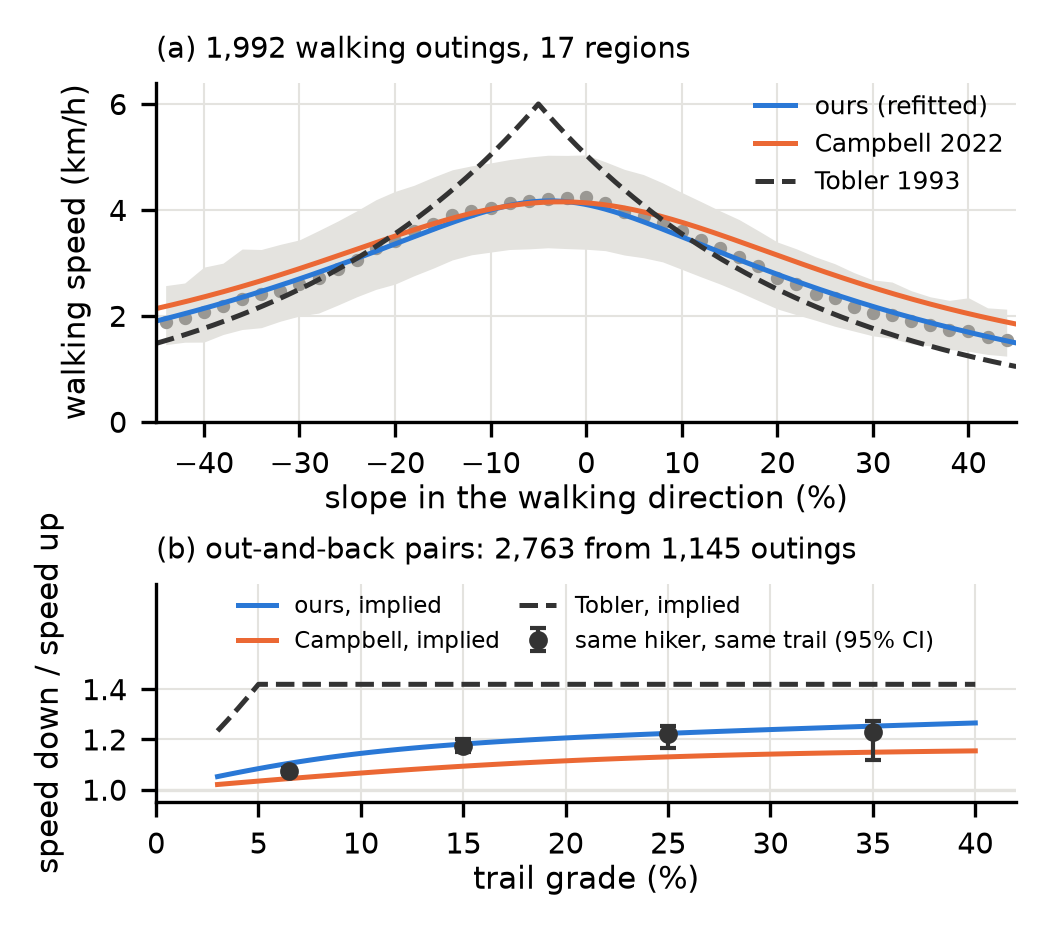
\includegraphics[width=\columnwidth]{fig_curve}
\caption{(a) Walking speed vs slope in the walking direction: median per
2\% bin (dots), middle 50\% of segments (gray), our refitted curve,
Campbell et al.'s median curve~\cite{campbell2022variability} and
Tobler's function~\cite{tobler1993}. (b) Speed down / speed up for the same
hiker on the same trail (out-and-back pairs; 95\% intervals resample
outings) and the ratio each curve implies.}
\label{fig:curve}
\end{figure}

\begin{figure*}[t]
\centering
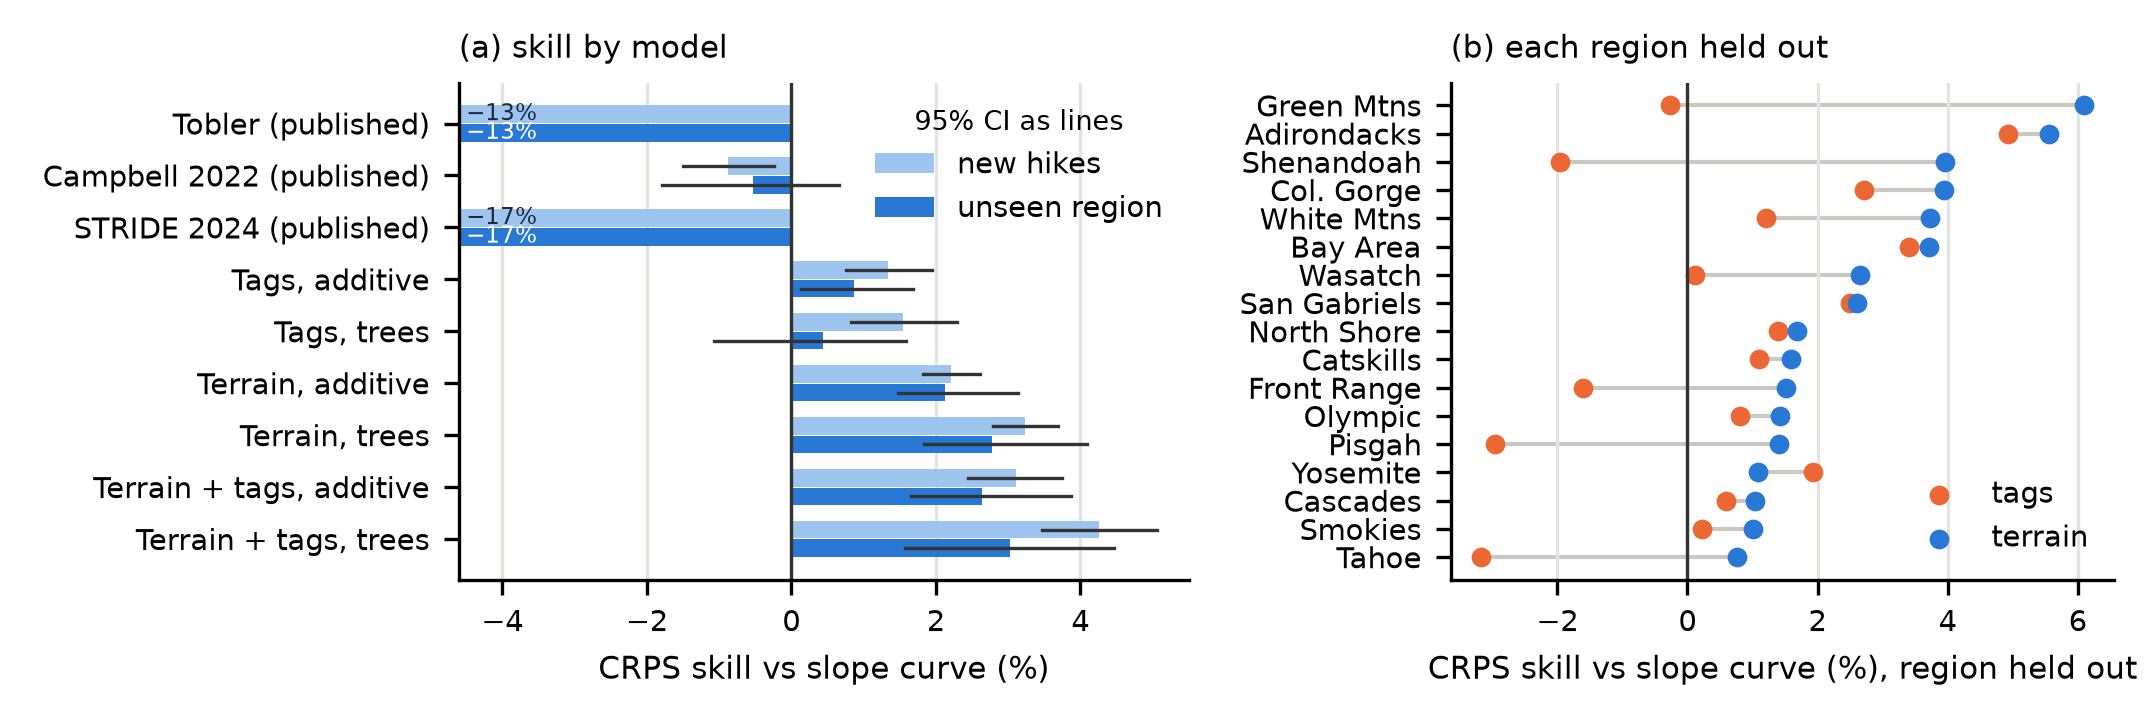
\includegraphics[width=\textwidth]{fig_skill_regions}
\caption{CRPS skill vs the refitted slope curve. (a) By model, for new
hikes in known regions (light; 95\% intervals resample outings) and in
regions the model never saw (dark; intervals resample regions). (b) Each
region held out:
terrain vs OSM tags (additive models); terrain beats tags in 16 of 17.}
\label{fig:skill}
\end{figure*}

% Dropped for the 4-page budget (paper/OUTLINE.md); restore if space allows:
% the travel-mode result (one shared curve x a constant per mode: runners
% x2.5 fine; bikes/skis ~4x walking downhill, ~1.6x uphill, own curve 3.8%
% lower RMSE; DECISIONS_LOG #96, #103);
% fig_hike_time.png (whole-hike time errors, R4) and fig_wm_pace.png (pace on
% every White Mountains trail, the practical output in the Discussion).
